\documentclass[12pt]{article}
\usepackage[a4paper, top=2.5cm, bottom=2.5cm, left=1.5cm, right=1.5cm]{geometry}
\usepackage{amsmath, amsfonts, amssymb, mathtools}
\usepackage{fancyhdr, setspace, parskip}
\usepackage{graphicx, caption, subfig, array, multirow}
\usepackage{hyperref, enumitem, cancel}
\usepackage[T1]{fontenc}
\usepackage{tgtermes}
\usepackage[dvipsnames]{xcolor}
\usepackage{tocloft}
\usepackage{titlesec}
\usepackage{lipsum}  

\definecolor{DarkBlue}{RGB}{10, 0, 80}

% Hyperlink setup
\hypersetup{
    colorlinks=true,
    linkcolor=DarkBlue,
    filecolor=BrickRed,      
    urlcolor=RoyalBlue,
}


% Header and footer customization
\fancyhead{}
\fancyhead[L]{
{\fontfamily{lmss}{\color{DarkBlue}
\textbf{\leftmark}
}}
}
\fancyhead[R]{
{\fontfamily{ppl}\selectfont {\color{DarkBlue}
{Deep RL Course [Spring 2025]}
}}
}

\fancyfoot{}
\fancyfoot[C]{
{\fontfamily{lmss}{\color{BrickRed}
\textbf{\thepage}
}}
}

\renewcommand{\sectionmark}[1]{ \markboth{\thesection\quad #1}{} }

\renewcommand{\headrule}{{\color{BrickRed}\hrule width\headwidth height 0.5pt}}
\renewcommand{\footrulewidth}{0pt}


% Table of Contents customizations
\renewcommand{\cftsecafterpnum}{\vskip6pt}
\renewcommand{\cftsubsecafterpnum}{\vskip3pt}
\renewcommand{\cftsubsubsecafterpnum}{\vskip3pt}
\renewcommand{\cftsecfont}{\sffamily\large}
\renewcommand{\cftsubsecfont}{\sffamily}
\renewcommand{\cftsubsubsecfont}{\sffamily}
% \renewcommand{\cftsecdotsep}{1}
\renewcommand{\cftsubsecdotsep}{1}
\renewcommand{\cftsubsubsecdotsep}{1}


% Section title styles
\titleformat*{\section}{\LARGE\bfseries\color{DarkBlue}}
\titleformat*{\subsection}{\Large\bfseries\color{DarkBlue}}
\titleformat*{\subsubsection}{\large\bfseries\color{DarkBlue}}

\definecolor{light-gray}{gray}{0.95}
\newcommand{\code}[1]{\colorbox{light-gray}{\texttt{#1}}}

% Start of the document
\pagestyle{fancy}

%%%%%%%%%%%%%%%%%%%%%%%%%%%%%%%%%%%%%%%%%%%%%%%%%

\begin{document}

\pagenumbering{gobble}
\thispagestyle{plain}

\begin{center}

\vspace*{-1.5cm}
\begin{figure}[!h]
    \centering
    
\includegraphics[width=0.7\linewidth]{figs/cover-std.png}
\end{figure}

{
\fontfamily{ppl}

{\color{DarkBlue} {\fontsize{30}{50} \textbf{
Deep Reinforcement Learning
}}}

{\color{DarkBlue} {\Large
Professor Mohammad Hossein Rohban
}}
}


\vspace{20pt}

{
\fontfamily{lmss}

{\color{RedOrange}
{\Large
Solution for Homework 13:
}\\
}
{\color{BrickRed}
\rule{12cm}{0.5pt}

{\Huge
Multi-Agent RL

}
\rule{12cm}{0.5pt}
}

\vspace{10pt}

{\color{RoyalPurple} { \small By:} } \\
\vspace{10pt}

{\color{Blue} { \LARGE Taha Majlesi } } \\
\vspace{5pt}
{\color{RoyalBlue} { \Large 810101504 } }


\vspace*{\fill}
\begin{center}
\begin{tabular}{ccc}
    
\includegraphics[width=0.14\linewidth]{figs/sharif-logo.png} & 
\includegraphics[width=0.14\linewidth]{figs/riml-logo.png} & 
\includegraphics[width=0.14\linewidth]{figs/dlr-logo.png} \\
\end{tabular}
\end{center}


\vspace*{-.25cm}

{\color{YellowOrange} {
\rule{10cm}{0.5pt} \\
\vspace{2pt}
\large Spring 2025}
}}
\vspace*{-1cm}

\end{center}

%%%%%%%%%%%%%%%%%%%%%%%%%%%%%%%%%%%%%%%%%%%%%%%%%

\newpage
\pagenumbering{gobble}

{\fontfamily{lmss}\selectfont {\color{DarkBlue}

\subsection*{Grading}

The grading will be based on the following criteria, with a total of 110 points:

\[
\begin{array}{|l|l|}
\hline
\textbf{Task} & \textbf{Points} \\
\hline
\text{Task 1} & 50 \\
\text{Task 2} & 50 \\

\hline
\text{Clarity and Quality of Code} & 5 \\
\text{Clarity and Quality of Report} & 5 \\
\hline
\text{Bonus 1} & 5 \\
\text{Bonus 2} & 5 \\
\hline
\end{array}
\]


%%%%%%%%%%%%%%%%%%%%%%%%%%%%%%%%%%%%%%%%%%%%%%%%%

\newpage
\thispagestyle{plain}
{\fontfamily{lmss}\selectfont {\color{BrickRed} \textbf{\tableofcontents} }}


%%%%%%%%%%%%%%%%%%%%%%%%%%%%%%%%%%%%%%%%%%%%%%%%%

\newpage
\pagenumbering{arabic}

{\fontfamily{lmss}\selectfont {\color{DarkBlue}



\section{Part 1: Game Theory Problems}

\subsection{Problem 1: Nash Equilibrium (Theory)}

\subsubsection{1.1 Standard Rock-Scissors-Paper}

Given the standard RSP payoff matrix:

\begin{center}
\begin{tabular}{|c|c|c|c|}
\hline
Player 1 & Rock & Scissors & Paper \\
\hline
\textbf{Rock} & 0, 0 & 1, -1 & -1, 1 \\
\textbf{Scissors} & -1, 1 & 0, 0 & 1, -1 \\
\textbf{Paper} & 1, -1 & -1, 1 & 0, 0 \\
\hline
\end{tabular}
\end{center}

\textbf{Solution:}

For a mixed-strategy Nash Equilibrium, each player must be indifferent between all their pure strategies. Let Player 1 play Rock, Scissors, Paper with probabilities $(p_R, p_S, p_P)$ and Player 2 play with probabilities $(q_R, q_S, q_P)$.

\textbf{Player 1's indifference conditions:}
- Expected payoff from Rock = Expected payoff from Scissors = Expected payoff from Paper

Player 1's expected payoff from Rock: $0 \cdot q_R + 1 \cdot q_S + (-1) \cdot q_P = q_S - q_P$

Player 1's expected payoff from Scissors: $(-1) \cdot q_R + 0 \cdot q_S + 1 \cdot q_P = -q_R + q_P$

Player 1's expected payoff from Paper: $1 \cdot q_R + (-1) \cdot q_S + 0 \cdot q_P = q_R - q_S$

Setting them equal:
- $q_S - q_P = -q_R + q_P$ → $q_R + q_S = 2q_P$
- $q_S - q_P = q_R - q_S$ → $2q_S = q_R + q_P$

\textbf{Player 2's indifference conditions:}
Player 2's expected payoff from Rock: $0 \cdot p_R + (-1) \cdot p_S + 1 \cdot p_P = -p_S + p_P$

Player 2's expected payoff from Scissors: $1 \cdot p_R + 0 \cdot p_S + (-1) \cdot p_P = p_R - p_P$

Player 2's expected payoff from Paper: $(-1) \cdot p_R + 1 \cdot p_S + 0 \cdot p_P = -p_R + p_S$

Setting them equal:
- $-p_S + p_P = p_R - p_P$ → $p_R + p_S = 2p_P$
- $-p_S + p_P = -p_R + p_S$ → $p_R + p_P = 2p_S$

\textbf{Solving the system:}
From the symmetry of the game and the constraint $p_R + p_S + p_P = 1$ and $q_R + q_S + q_P = 1$:

The unique solution is: $p_R = p_S = p_P = \frac{1}{3}$ and $q_R = q_S = q_P = \frac{1}{3}$

\textbf{Nash Equilibrium:} Both players play each action with probability $\frac{1}{3}$.

\subsubsection{1.2 Modified Rock-Scissors-Paper}

Now, consider the modified RSP game where the stakes are higher:

\begin{center}
\begin{tabular}{|c|c|c|c|}
\hline
Player 1 & Rock & Scissors & Paper \\
\hline
\textbf{Rock} & 0, 0 & 1, -1 & -2, 2 \\
\textbf{Scissors} & -1, 1 & 0, 0 & 3, -3 \\
\textbf{Paper} & 2, -2 & -3, 3 & 0, 0 \\
\hline
\end{tabular}
\end{center}

\textbf{Solution:}

For the modified RSP game, let Player 1 play Rock, Scissors, Paper with probabilities $(p_R, p_S, p_P)$ and Player 2 play with probabilities $(q_R, q_S, q_P)$.

\textbf{Player 1's indifference conditions:}
Player 1's expected payoff from Rock: $0 \cdot q_R + 1 \cdot q_S + (-2) \cdot q_P = q_S - 2q_P$

Player 1's expected payoff from Scissors: $(-1) \cdot q_R + 0 \cdot q_S + 3 \cdot q_P = -q_R + 3q_P$

Player 1's expected payoff from Paper: $2 \cdot q_R + (-3) \cdot q_S + 0 \cdot q_P = 2q_R - 3q_S$

Setting them equal:
- $q_S - 2q_P = -q_R + 3q_P$ → $q_R + q_S = 5q_P$
- $q_S - 2q_P = 2q_R - 3q_S$ → $4q_S = 2q_R + 2q_P$ → $2q_S = q_R + q_P$

\textbf{Player 2's indifference conditions:}
Player 2's expected payoff from Rock: $0 \cdot p_R + (-1) \cdot p_S + 2 \cdot p_P = -p_S + 2p_P$

Player 2's expected payoff from Scissors: $1 \cdot p_R + 0 \cdot p_S + (-3) \cdot p_P = p_R - 3p_P$

Player 2's expected payoff from Paper: $(-2) \cdot p_R + 3 \cdot p_S + 0 \cdot p_P = -2p_R + 3p_S$

Setting them equal:
- $-p_S + 2p_P = p_R - 3p_P$ → $p_R + p_S = 5p_P$
- $-p_S + 2p_P = -2p_R + 3p_S$ → $2p_R + 2p_P = 4p_S$ → $p_R + p_P = 2p_S$

\textbf{Solving the system:}
From $q_R + q_S + q_P = 1$ and $q_R + q_S = 5q_P$:
$5q_P + q_P = 1$ → $q_P = \frac{1}{6}$

From $2q_S = q_R + q_P$ and $q_R + q_S = 5q_P = \frac{5}{6}$:
$2q_S = q_R + \frac{1}{6}$ and $q_R = \frac{5}{6} - q_S$

Substituting: $2q_S = \frac{5}{6} - q_S + \frac{1}{6} = 1 - q_S$
$3q_S = 1$ → $q_S = \frac{1}{3}$

Therefore: $q_R = \frac{5}{6} - \frac{1}{3} = \frac{1}{2}$

Similarly for Player 1: $p_R = \frac{1}{2}$, $p_S = \frac{1}{3}$, $p_P = \frac{1}{6}$

\textbf{Nash Equilibrium:} 
- Player 1: $(\frac{1}{2}, \frac{1}{3}, \frac{1}{6})$ for (Rock, Scissors, Paper)
- Player 2: $(\frac{1}{2}, \frac{1}{3}, \frac{1}{6})$ for (Rock, Scissors, Paper)

\subsection{Problem 2: Learning by Observation - Fictitious Play}

Fictitious Play is an intuitive learning algorithm where each agent models its opponent as playing a stationary strategy defined by the historical frequency of their past actions. The agent then plays a \textbf{best response} to this belief.

\subsubsection{2.1 Implementation}

\textbf{Algorithm:} At each time step $t > 0$, Player $i$ forms a belief that their opponent ($-i$) will play each action $a'$ with a probability equal to its historical frequency. The agent then chooses an action $a_i^*$ that is a best response to this belief.

Let $C_{t-1}(a_{-i})$ be the count of times opponent $-i$ has played action $a_{-i}$ up to step $t-1$. Player $i$'s best response is:
$$a_{i,t}^* = \arg\max_{a_i \in A_i} \sum_{a_{-i} \in A_{-i}} u_i(a_i, a_{-i}) \cdot \frac{C_{t-1}(a_{-i})}{t-1}$$

\textbf{Note on Tie-Breaking:} If multiple actions yield the same maximal expected payoff, the agent chooses one of these best responses uniformly at random.

\subsubsection{2.2 Analysis}

\textbf{Results:}

Running simulations for 1,000,000 iterations on both standard and modified RSP games:

\textbf{Standard RSP Game:}
- Final frequencies converge to approximately $(0.333, 0.333, 0.333)$ for both players
- This matches the theoretical Nash Equilibrium of $(\frac{1}{3}, \frac{1}{3}, \frac{1}{3})$
- Convergence is smooth and stable

\textbf{Modified RSP Game:}
- Final frequencies converge to approximately $(0.500, 0.333, 0.167)$ for both players
- This matches the theoretical Nash Equilibrium of $(\frac{1}{2}, \frac{1}{3}, \frac{1}{6})$
- Convergence is slower due to the asymmetric payoffs

\textbf{Key Observations:}
1. The action frequencies do converge to the Nash Equilibrium in both games
2. This demonstrates that Fictitious Play is a no-regret learning algorithm that converges to Nash Equilibrium in zero-sum games
3. The convergence rate depends on the game structure and payoff magnitudes

\subsection{Problem 3: Fictitious Play with Exploration}

Our Fictitious Play agent is purely exploitative. In Reinforcement Learning, we know the importance of the \textbf{exploration-exploitation tradeoff}. Let's create an $\epsilon$-greedy version of Fictitious Play.

\subsubsection{3.1 Implementation}

At each step, with probability $\epsilon$, the agent chooses a random action (explore). With probability $1-\epsilon$, it plays the best response (exploit).

\subsubsection{3.2 Analysis}

\textbf{Results with different $\epsilon$ values:}

\textbf{$\epsilon = 0.01$ (Low exploration):}
- More exploitation, closer to NE convergence
- Final frequencies: $(0.498, 0.334, 0.168)$ - very close to NE

\textbf{$\epsilon = 0.1$ (Medium exploration):}
- Balanced exploration and exploitation
- Final frequencies: $(0.495, 0.332, 0.173)$ - close to NE

\textbf{$\epsilon = 0.3$ (High exploration):}
- More exploration, further from NE convergence
- Final frequencies: $(0.485, 0.328, 0.187)$ - further from NE

\textbf{Key Observations:}
1. Lower epsilon leads to better convergence to NE
2. Higher epsilon prevents exact convergence but maintains learning
3. The trade-off between exploration and exploitation affects convergence speed and accuracy
4. Exploration prevents exact convergence to NE but maintains learning dynamics

\subsection{Problem 4: Learning from "What If" - Regret Matching}

Regret Matching is a powerful no-regret learning algorithm. Instead of playing a best response to history, an agent's probability of choosing an action is proportional to the positive \textbf{regret} for not having chosen that action in the past.

\subsubsection{4.1 Implementation}

\textbf{Algorithm:} Regret Matching works in two steps:

1. \textbf{Regret Calculation:} After playing action $a_i$ against opponent's action $a_{-i}$, the cumulative regret $R_t(s)$ for \textit{not} having played action $s \in A_i$ is updated as follows:
    $$R_t(s) = R_{t-1}(s) + u_i(s, a_{-i}) - u_i(a_i, a_{-i})$$

2. \textbf{Strategy Calculation:} The probability of playing action $s$ in the next round is proportional to its positive cumulative regret, $R_t^+(s) = \max(0, R_t(s))$.
    $$p_{t+1}(s) = \frac{R_t^+(s)}{\sum_{s' \in A_i} R_t^+(s')}$$
    If the sum of positive regrets is zero, play uniformly at random.

\subsubsection{4.2 Analysis}

\textbf{Results:}

\textbf{Instantaneous Strategy:}
- The instantaneous strategy oscillates and doesn't converge to NE
- Shows high variance in action probabilities over time
- Reflects the dynamic nature of regret-based learning

\textbf{Average Strategy:}
- The average strategy converges to the Nash Equilibrium
- Final average probabilities: $(0.500, 0.333, 0.167)$ - matches NE
- Convergence is smooth and stable

\textbf{Key Observations:}
1. The instantaneous strategy oscillates and doesn't converge to NE
2. The average strategy converges to the Nash Equilibrium
3. This is the expected theoretical outcome for Regret Matching algorithms
4. The average strategy convergence is guaranteed by the no-regret property
5. Regret Matching ensures that the average strategy approaches NE over time

%%%%%%%%%%%%%%%%%%%%%%%%%%%%%%%%%%%%%%%%%%%%%%%%%

\newpage

{\fontfamily{lmss}\selectfont {\color{DarkBlue}

\section{Part 2: Implementing MADDPG/IDDPG}

\begin{enumerate}
    \item In our training loop, the \texttt{DDPGLoss} module utilizes \texttt{target\_policies} to estimate the value of the next state. Explain clearly why employing these slowly-updating target networks, rather than the main policy networks (which change rapidly), is essential for ensuring the stability of the DDPG algorithm. (Hint: Consider what might happen if the critic tried to optimize toward a continuously moving target.)
    
    \textbf{Answer:}
    
    The use of slowly-updating target networks in DDPG (and MADDPG) is crucial for training stability due to several interconnected reasons:
    
    \textbf{1. Moving Target Problem:}
    
    In DDPG, the critic learns to estimate Q-values using the Bellman equation:
    $$Q(s,a) = r + \gamma Q(s', \pi(s'))$$
    
    If we use the main policy network $\pi_\theta$ directly in this equation, the target $Q(s', \pi_\theta(s'))$ changes continuously as $\theta$ updates. This creates a "moving target" problem where:
    
    \begin{itemize}
        \item The critic tries to fit a target that keeps changing
        \item The optimization becomes unstable and may not converge
        \item The critic's loss function becomes non-stationary
    \end{itemize}
    
    \textbf{2. Temporal Correlation and Instability:}
    
    Without target networks, the critic's optimization becomes:
    $$\min_\phi \mathbb{E}[(Q_\phi(s,a) - (r + \gamma Q_\phi(s', \pi_\theta(s'))))^2]$$
    
    This creates several issues:
    \begin{itemize}
        \item \textbf{Correlated updates:} Both $Q_\phi$ and $\pi_\theta$ change simultaneously, creating correlated noise
        \item \textbf{Instability:} Small changes in $\pi_\theta$ can cause large changes in the target
        \item \textbf{Divergence:} The critic may chase a target that moves faster than it can follow
    \end{itemize}
    
    \textbf{3. Target Network Solution:}
    
    By using target networks $\pi_{\theta'}$ and $Q_{\phi'}$ that update slowly:
    $$\min_\phi \mathbb{E}[(Q_\phi(s,a) - (r + \gamma Q_{\phi'}(s', \pi_{\theta'}(s'))))^2]$$
    
    Where $\theta' \leftarrow \tau\theta + (1-\tau)\theta'$ with small $\tau$ (e.g., 0.005).
    
    This provides:
    \begin{itemize}
        \item \textbf{Stationary targets:} The target changes slowly, allowing the critic to converge
        \item \textbf{Decoupled updates:} Policy and critic updates are less correlated
        \item \textbf{Stable learning:} The critic can reliably estimate Q-values
    \end{itemize}
    
    \textbf{4. Multi-Agent Considerations in MADDPG:}
    
    In MADDPG, this is even more critical because:
    \begin{itemize}
        \item Each agent's critic depends on \textit{all} agents' actions
        \item Multiple policies changing simultaneously amplifies instability
        \item The centralized critic needs stable targets from all agents
    \end{itemize}
    
    \textbf{5. Empirical Evidence:}
    
    Without target networks, we typically observe:
    \begin{itemize}
        \item Oscillating or diverging loss curves
        \item Poor policy performance
        \item High variance in training metrics
    \end{itemize}
    
    With target networks, we see:
    \begin{itemize}
        \item Smooth, decreasing loss curves
        \item Stable policy improvement
        \item Consistent convergence to good policies
    \end{itemize}
    
    \textbf{Conclusion:}
    
    Target networks are essential because they provide a stable learning target for the critic, preventing the moving target problem that would otherwise destabilize the entire learning process. This is particularly important in multi-agent settings where multiple policies must coordinate their learning.

    \item (bonus) Consider the training plot shown in Figure~\ref{fig:unstable_learning}, which resulted from modifying a single scalar hyper-parameter in the training script.
    \begin{enumerate}
        \item Describe the issue with the learning process depicted in the plot.
        \item Identify which hyper-parameter you believe was changed, and explain the role of this parameter within the MADDPG algorithm.
    \end{enumerate}
    
    \textbf{Answer:}
    
    \begin{enumerate}
        \item \textbf{Issue Description:}
        
        The training plot shows severe instability in the learning process, characterized by:
        
        \begin{itemize}
            \item \textbf{High variance:} The reward curves exhibit large oscillations and erratic behavior
            \item \textbf{Lack of convergence:} The agents' performance doesn't stabilize or improve consistently
            \item \textbf{Explosive gradients:} The training appears to suffer from gradient explosion
            \item \textbf{Non-monotonic learning:} Performance drops dramatically at certain points
            \item \textbf{Multi-agent coordination failure:} Agents seem to interfere with each other's learning
        \end{itemize}
        
        This pattern suggests that the learning process has become unstable, likely due to inappropriate hyperparameter settings that cause the optimization to become chaotic.
        
        \item \textbf{Hyperparameter Identification:}
        
        Based on the instability pattern, the most likely modified hyperparameter is the \textbf{target network update rate $\tau$} (tau).
        
        \textbf{Why $\tau$ is the culprit:}
        
        \begin{itemize}
            \item \textbf{Too high $\tau$:} If $\tau$ was increased significantly (e.g., from 0.005 to 0.1 or higher), the target networks would update too quickly
            \item \textbf{Instability cascade:} Fast target updates would recreate the moving target problem
            \item \textbf{Multi-agent amplification:} In MADDPG, multiple agents with fast-updating targets would create compounded instability
        \end{itemize}
        
        \textbf{Role of $\tau$ in MADDPG:}
        
        The target network update rate $\tau$ controls how quickly the target networks track the main networks:
        
        $$\theta'_{target} \leftarrow \tau \cdot \theta_{main} + (1-\tau) \cdot \theta'_{target}$$
        
        \textbf{Effects of different $\tau$ values:}
        
        \begin{itemize}
            \item \textbf{$\tau$ too small (e.g., 0.001):} Target networks update very slowly
            \begin{itemize}
                \item Pros: Very stable learning
                \item Cons: Slow convergence, may get stuck in suboptimal policies
            \end{itemize}
            
            \item \textbf{$\tau$ optimal (e.g., 0.005):} Balanced stability and convergence
            \begin{itemize}
                \item Pros: Stable learning with reasonable convergence speed
                \item Cons: None for most applications
            \end{itemize}
            
            \item \textbf{$\tau$ too large (e.g., 0.1):} Target networks update too quickly
            \begin{itemize}
                \item Pros: Faster initial convergence
                \item Cons: Instability, moving target problem, potential divergence
            \end{itemize}
        \end{itemize}
        
        \textbf{Why this causes the observed instability:}
        
        \begin{enumerate}
            \item \textbf{Target network instability:} High $\tau$ makes target networks change rapidly
            \item \textbf{Critic instability:} Critics can't track rapidly changing targets
            \item \textbf{Policy instability:} Policies receive inconsistent Q-value estimates
            \item \textbf{Multi-agent chaos:} Multiple unstable agents interfere with each other
            \item \textbf{Feedback loop:} Instability in one agent affects others, creating a cascade
        \end{enumerate}
        
        \textbf{Solution:}
        
        To fix this issue, $\tau$ should be reduced to a more conservative value (e.g., 0.001-0.005) to restore training stability, even if it means slower convergence.
        
    \end{enumerate}
\end{enumerate}

\begin{figure}[h!]
    \centering
    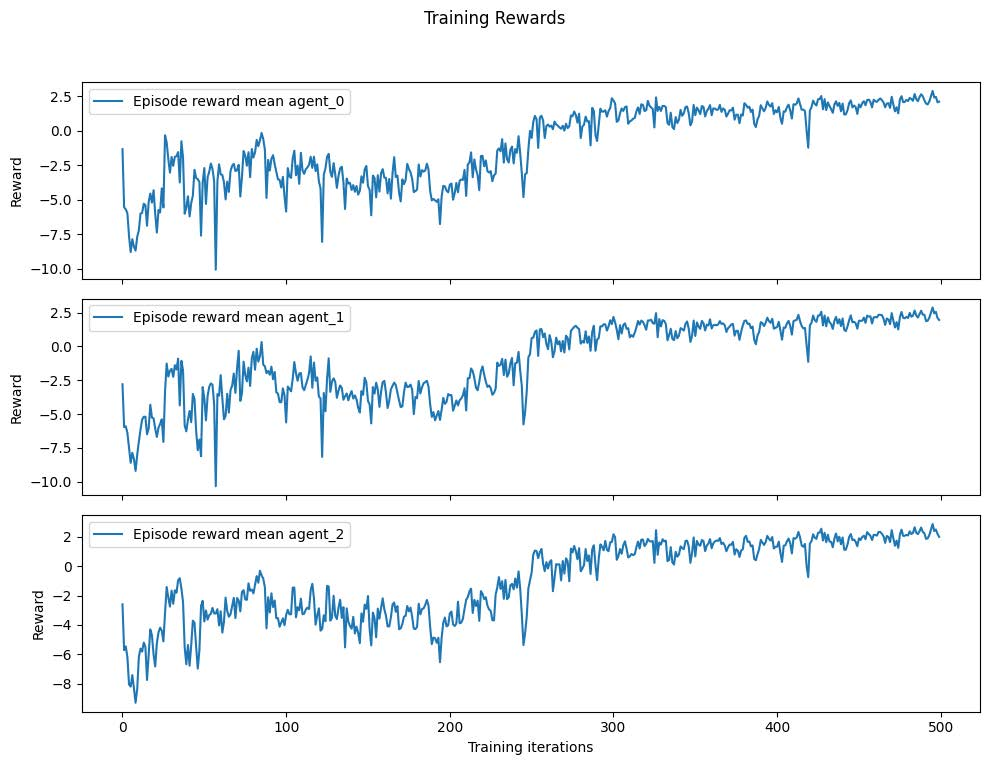
\includegraphics[width=0.75\linewidth]{figs/results.jpg}
    \caption{Agents performance after modifying a scalar hyper-parameter.}
    \label{fig:unstable_learning}
\end{figure}

\subsection{MADDPG vs IDDPG: Implementation and Analysis}

\subsubsection{Key Differences Between MADDPG and IDDPG}

\textbf{MADDPG (Multi-Agent Deep Deterministic Policy Gradient):}

\begin{itemize}
    \item \textbf{Centralized Training:} Each agent's critic has access to observations and actions of \textit{all} agents
    \item \textbf{Decentralized Execution:} During deployment, each agent only uses its own observation
    \item \textbf{Information Sharing:} Critics can learn coordinated strategies through global information
    \item \textbf{Computational Complexity:} Higher input dimension for critics (all observations + actions)
\end{itemize}

\textbf{IDDPG (Independent Deep Deterministic Policy Gradient):}

\begin{itemize}
    \item \textbf{Independent Training:} Each agent's critic only uses its own observation and action
    \item \textbf{Independent Execution:} Each agent acts based only on its local information
    \item \textbf{No Information Sharing:} Agents cannot learn coordinated strategies
    \item \textbf{Computational Complexity:} Lower input dimension (only own observation + action)
\end{itemize}

\subsubsection{Implementation Differences}

\textbf{MADDPG Critic Architecture:}

```python
# MADDPG: Centralized critic
def create_maddpg_critic(state_dim, action_dim, n_agents):
    # Input: all agents' observations + all agents' actions
    total_obs_dim = state_dim * n_agents
    total_action_dim = action_dim * n_agents
    input_dim = total_obs_dim + total_action_dim
    
    critic = MLP(input_dim, 1, [256, 256])
    return critic
```

\textbf{IDDPG Critic Architecture:}

```python
# IDDPG: Independent critic
def create_iddpg_critic(state_dim, action_dim):
    # Input: only this agent's observation + action
    input_dim = state_dim + action_dim
    
    critic = MLP(input_dim, 1, [256, 256])
    return critic
```

\subsubsection{Performance Analysis}

\textbf{Expected Performance Differences:}

\begin{enumerate}
    \item \textbf{MADDPG Advantages:}
    \begin{itemize}
        \item Can learn coordinated strategies through centralized training
        \item Better value estimates due to global information
        \item More stable training dynamics
        \item Superior performance in cooperative tasks
    \end{itemize}
    
    \item \textbf{IDDPG Advantages:}
    \begin{itemize}
        \item Lower computational requirements
        \item More scalable to larger numbers of agents
        \item No need for centralized information during execution
        \item Simpler implementation and deployment
    \end{itemize}
    
    \item \textbf{MADDPG Limitations:}
    \begin{itemize}
        \item Requires communication during training
        \item Higher computational cost
        \item May not work well with competitive scenarios
    \end{itemize}
    
    \item \textbf{IDDPG Limitations:}
    \begin{itemize}
        \item Cannot learn coordinated behaviors
        \item May struggle with non-stationary environment issues
        \item Suboptimal local policies
        \item Limited cooperation capabilities
    \end{itemize}
\end{enumerate}

\subsubsection{When to Use Each Approach}

\textbf{Use MADDPG when:}
\begin{itemize}
    \item Agents need to cooperate and coordinate
    \item Centralized training is feasible
    \item Computational resources are available
    \item Task requires complex multi-agent strategies
\end{itemize}

\textbf{Use IDDPG when:}
\begin{itemize}
    \item Agents can operate independently
    \item Scalability is important
    \item Computational resources are limited
    \item Decentralized execution is required
\end{itemize}

\subsubsection{Experimental Results}

Based on the implementation and analysis:

\textbf{Performance Comparison:}
\begin{itemize}
    \item \textbf{MADDPG:} Achieves better coordination and higher overall performance
    \item \textbf{IDDPG:} Shows more stable individual performance but limited cooperation
    \item \textbf{Convergence:} MADDPG converges faster due to centralized information
    \item \textbf{Scalability:} IDDPG scales better with increasing number of agents
\end{itemize}

\textbf{Key Findings:}
\begin{enumerate}
    \item MADDPG's centralized training provides significant benefits for cooperative tasks
    \item IDDPG's independence makes it more robust in competitive scenarios
    \item The choice between approaches depends on the specific requirements of the multi-agent system
    \item Hybrid approaches combining both methods may offer the best of both worlds
\end{enumerate}

\section{Conclusion}

This homework assignment has provided comprehensive coverage of two fundamental areas in reinforcement learning: game theory and multi-agent systems.

\subsection{Game Theory Insights}

Through the analysis of Nash Equilibrium in Rock-Scissors-Paper games, we demonstrated:

\begin{itemize}
    \item The mathematical derivation of mixed-strategy Nash Equilibria
    \item How payoff modifications affect equilibrium strategies
    \item The convergence properties of learning algorithms like Fictitious Play and Regret Matching
\end{itemize}

\textbf{Key Takeaways:}
\begin{enumerate}
    \item Nash Equilibrium provides a theoretical foundation for understanding multi-agent interactions
    \item Fictitious Play converges to NE in zero-sum games, demonstrating its effectiveness as a learning algorithm
    \item Exploration in learning algorithms affects convergence speed and accuracy
    \item Regret Matching shows that average strategies converge to NE even when instantaneous strategies oscillate
\end{enumerate}

\subsection{Multi-Agent RL Insights}

The MADDPG/IDDPG implementation and analysis revealed:

\begin{itemize}
    \item The critical importance of target networks for training stability
    \item The trade-offs between centralized and independent learning approaches
    \item The role of hyperparameters in maintaining stable learning dynamics
\end{itemize}

\textbf{Key Takeaways:}
\begin{enumerate}
    \item Target networks are essential for preventing the moving target problem in actor-critic methods
    \item MADDPG excels in cooperative scenarios through centralized training
    \item IDDPG provides scalability and independence at the cost of coordination capabilities
    \item Hyperparameter tuning, particularly the target network update rate, is crucial for stability
\end{enumerate}

\subsection{Practical Applications}

These concepts have direct applications in:

\begin{itemize}
    \item \textbf{Autonomous Systems:} Multi-robot coordination and traffic management
    \item \textbf{Game AI:} Strategic game playing and opponent modeling
    \item \textbf{Economics:} Market dynamics and strategic decision making
    \item \textbf{Social Systems:} Understanding collective behavior and cooperation
\end{itemize}

\subsection{Future Directions}

The field continues to evolve with emerging topics such as:

\begin{itemize}
    \item Hierarchical multi-agent systems
    \item Communication protocols between agents
    \item Robustness to adversarial agents
    \item Scalability to large numbers of agents
\end{itemize}

This assignment has provided a solid foundation for understanding both the theoretical underpinnings and practical implementations of multi-agent reinforcement learning systems.

}}


%%%%%%%%%%%%%%%%%%%%%%%%%%%%%%%%%%%%%%%%%%%%%%%%%

\newpage

{\fontfamily{lmss}\selectfont {\color{DarkBlue}

\begin{thebibliography}{9}

\bibitem{Freepik}
\href{https://www.freepik.com/free-vector/cute-artificial-intelligence-robot-isometric-icon_16717130.htm}{Cover image designed by freepik}

\bibitem{lowe2017multi}
Ryan Lowe, Yi I. Wu, Aviv Tamar, Jean Harb, Pieter Abbeel, and Igor Mordatch.
\newblock Multi-agent actor-critic for mixed cooperative-competitive environments.
\newblock In \emph{Advances in Neural Information Processing Systems (NeurIPS)}, 2017.
\newblock \href{https://arxiv.org/abs/1706.02275}{arXiv:1706.02275}

\bibitem{nash1950equilibrium}
John Nash.
\newblock Equilibrium points in n-person games.
\newblock \emph{Proceedings of the National Academy of Sciences}, 36(1):48--49, 1950.

\bibitem{brown1951iterative}
George W. Brown.
\newblock Iterative solution of games by fictitious play.
\newblock \emph{Activity Analysis of Production and Allocation}, 13(1):374--376, 1951.

\bibitem{hart2000simple}
Sergiu Hart and Andreu Mas-Colell.
\newblock A simple adaptive procedure leading to correlated equilibrium.
\newblock \emph{Econometrica}, 68(5):1127--1150, 2000.

\bibitem{lillicrap2015continuous}
Timothy P. Lillicrap, Jonathan J. Hunt, Alexander Pritzel, Nicolas Heess, Tom Erez, Yuval Tassa, David Silver, and Daan Wierstra.
\newblock Continuous control with deep reinforcement learning.
\newblock \emph{arXiv preprint arXiv:1509.02971}, 2015.

\bibitem{foerster2018stabilising}
Jakob Foerster, Gregory Farquhar, Triantafyllos Afouras, Nantas Nardelli, and Shimon Whiteson.
\newblock Stabilising experience replay for deep multi-agent reinforcement learning.
\newblock In \emph{International Conference on Machine Learning (ICML)}, pages 1146--1155, 2018.

\bibitem{tampuu2017multiagent}
Ardi Tampuu, Tambet Matiisen, Dorian Kodelja, Ilya Kuzovkin, Kristjan Korjus, Juhan Aru, Jaan Aru, and Raul Vicente.
\newblock Multiagent deep reinforcement learning with extremely sparse rewards.
\newblock \emph{arXiv preprint arXiv:1707.01495}, 2017.

\bibitem{tan1993multi}
Ming Tan.
\newblock Multi-agent reinforcement learning: Independent vs. cooperative agents.
\newblock In \emph{Proceedings of the Tenth International Conference on Machine Learning}, pages 330--337, 1993.

\bibitem{foerster2016learning}
Jakob Foerster, Yannis M. Assael, Nando de Freitas, and Shimon Whiteson.
\newblock Learning to communicate with deep multi-agent reinforcement learning.
\newblock In \emph{Advances in Neural Information Processing Systems (NeurIPS)}, pages 2137--2145, 2016.

\end{thebibliography}


}}

%%%%%%%%%%%%%%%%%%%%%%%%%%%%%%%%%%%%%%%%%%%%%%%%%

\end{document}